% Chapter 1

\chapter{Organisation de l'équipe et planning} % Main chapter title

\label{Chapter1} % For referencing the chapter elsewhere, use \ref{Chapter1}

%----------------------------------------------------------------------------------------

\section{Organisation de l'équipe}

Afin de se concentrer sur la "Solution n°2" lundi 8 nous nous sommes lancés dans
l'annalyse du code c du driver et du déroulé de son fonctionnement.

Par la suite Romain suivi par Alan se sont lancés dans le second objectif
d'évolution, la compilation d'un noyau en version 4.14. Ce afinde précéder le
portage du driver à ce kernel.

\begin{comment}
\section{Planning}

Nous vous avons ici présenté un planning des tâches effectuées durant ces 8 \\
derniers jours, les noms attribués à chaque tâche seront développés dans la suite du rapport.

%\begin{figure}[th]
%    \centering
%    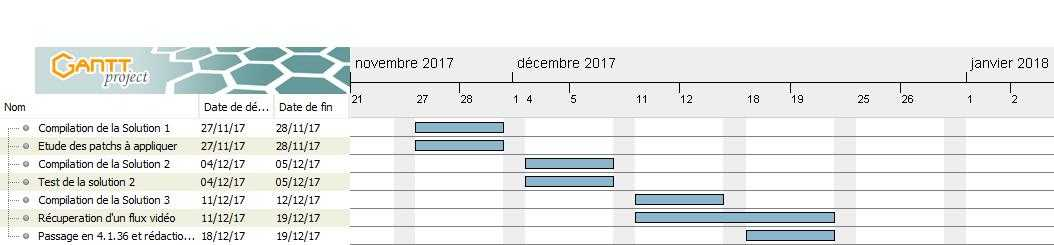
\includegraphics[width=1\linewidth]{planning.png}
%    \decoRule
%    \caption{Avancement du projet actuel}  \label{fig:planning}
%\end{figure}

Les trois solutions qui sont présentées ci-dessous correspondent à trois codes sources.

%----------------------------------------------------------------------------------------
\end{comment}
